\documentclass[10pt,tumble]{leaflet}
\usepackage[T1]{fontenc}
\usepackage{libertine}
\renewcommand{\familydefault}{\sfdefault}
\usepackage{microtype}
\usepackage{graphicx}
\usepackage{float}
\pagenumbering{gobble}

\title{Team 2767}
\author{\Large\textbf{Stryke Force}}

\begin{document}
\begin{center}
 \LARGE\textbf{Team 2767\\ Stryke Force}\\
 \Large{Est. 2009\\ Kalamazoo, MI}\\
 \vspace{0.5in}
 
\includegraphics[scale=0.2]{assets/strykeforce}\\
 \vspace{0.5in}
 \LARGE\textbf{Software Development Team 2019}\vspace{0.5in}\\ \textit{FIRST}\textregistered DESTINATION: DEEP SPACE Presented By The Boeing Company \vspace{0.25in} \\ {\large www.strykeforce.org\\www.github.com/strykeforce}
 \vfill
\end{center}
\clearpage

\section{Software Designed for Drivers}
Stryke Force is proud to present the control system software for \textbf{Air Tight}, our robot competing in \textit{FIRST}\textregistered DESTINATION: DEEP SPACE Presented By The Boeing Company.

We strive to meld high-performance hardware with custom software to provide our drive team with the best robot possible. Our \textbf{Third Coast Swerve Drive} software has historically provided unmatched maneuverability and response.

\section{Precision Control Systems}

Stryke Force delved deep into motion profiling this year.  Using the \textbf{CTR-Electronics Talon SRX Motion Magic} functionality, the programming team controls the motion-profile using acceleration, velocity, current limit, and PID parameters.  This feature in the software allows the robot to make precise and repeatable movements in all subsystems.

\section{``Robot Safety Glasses''}

\begin{figure}[H]
	\centering
	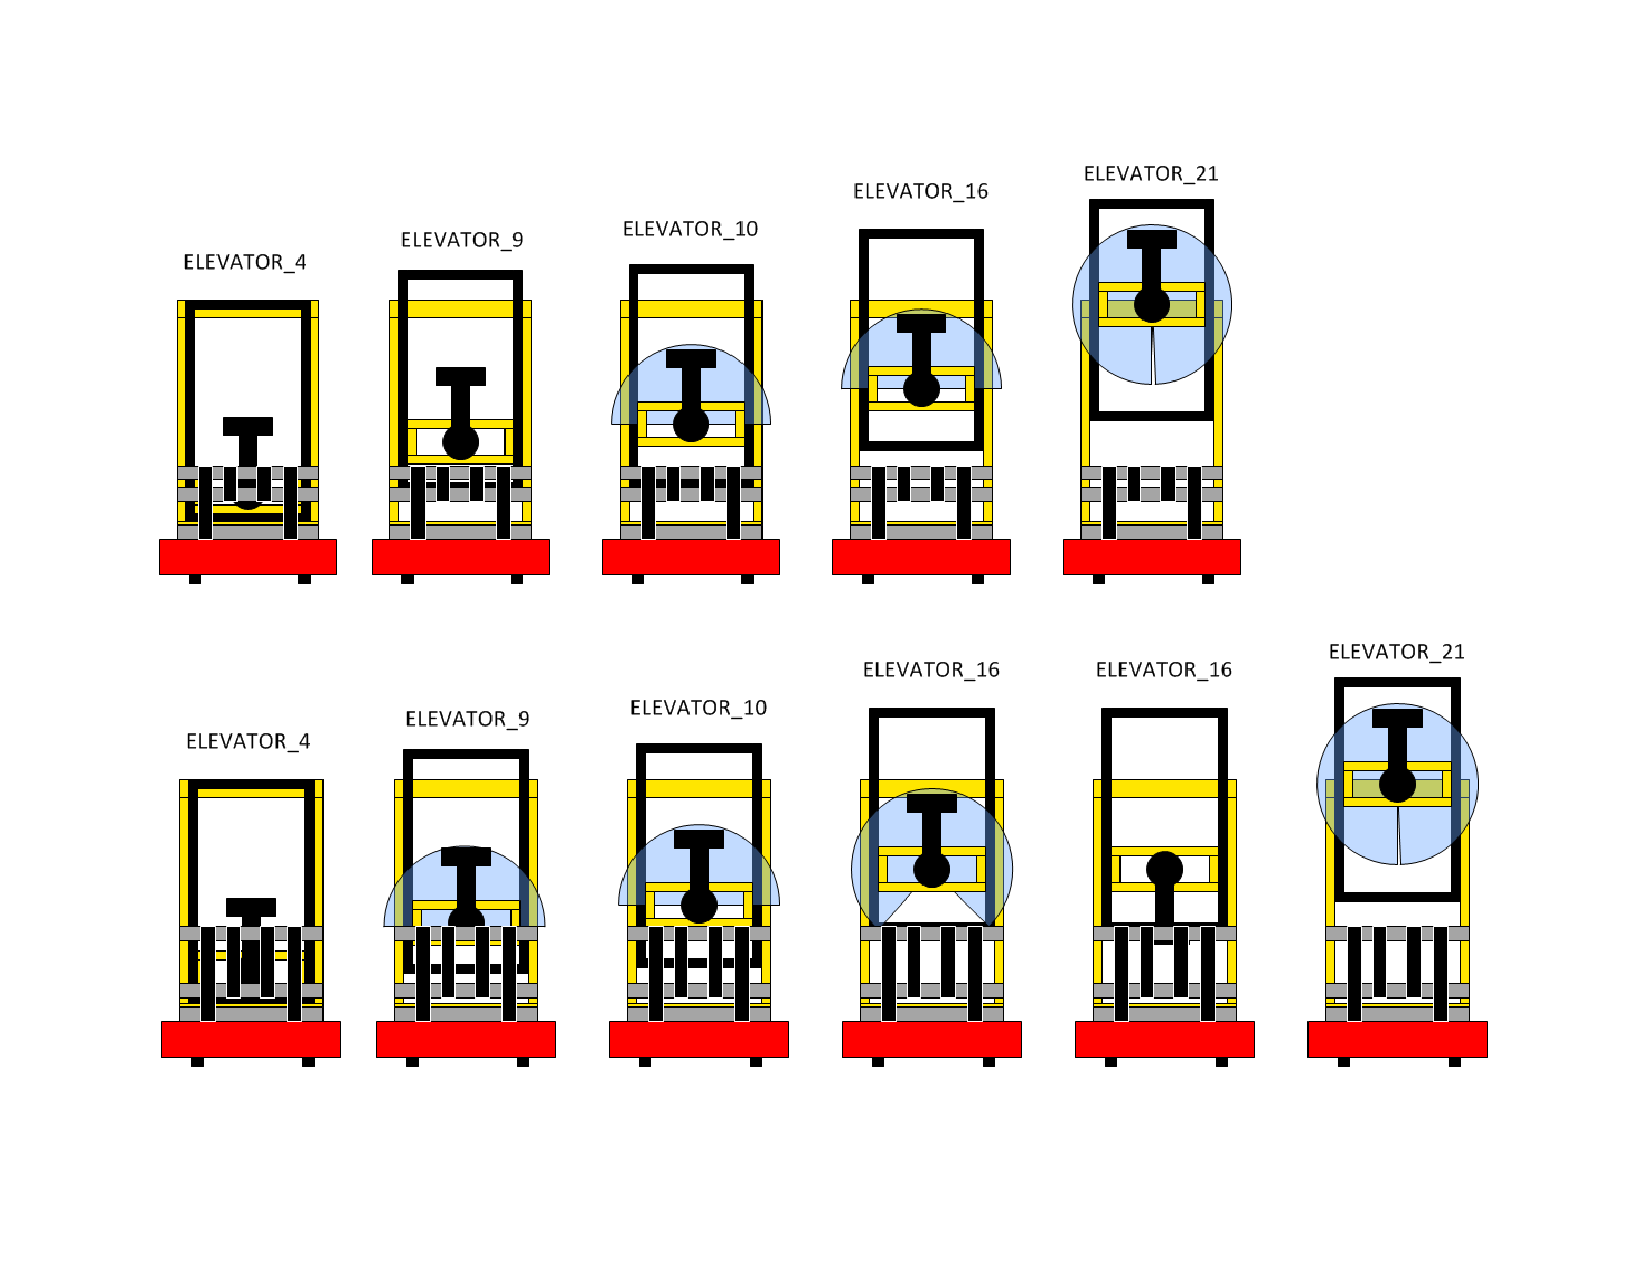
\includegraphics[scale=0.3]{assets/safety}
\end{figure}

At Stryke Force, safety is our primary concern so it's only natural that safety rules apply to all, human and otherwise: robot. Programmers are using a custom \textbf{Safety Subsystem} that interfaces with the Elevator, Biscuit (arm rotation), and Intake subsystems. Every 20ms, all three subsystems update their current state and then the Safety Subsystem runs through a matrix of legal and safe positions updating Talon SRX forward and reverse soft limits. Since the axes cannot pass the soft limits, the programmers ensure the robot's safety.

\section{``Twisting our way through the sandstorm''}

\begin{figure}[H]
	\centering
	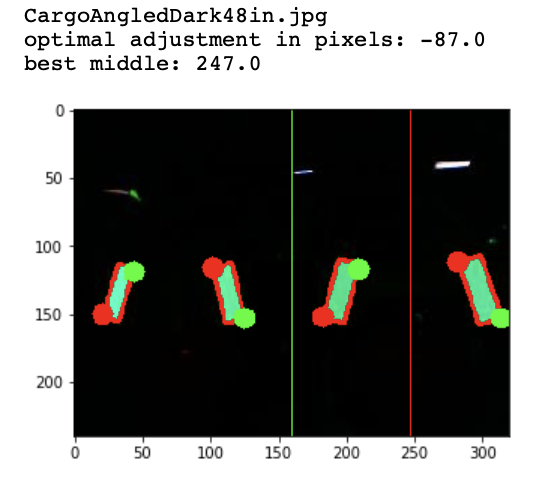
\includegraphics[scale=0.75]{assets/vision}
\end{figure}

The software team focused on helping our driver perform during Sandstorm. In addition to pathfinding using Pathfinder, we're implementing \textbf{computer vision} (CV) to guide our driver through Sandstorm. Since vision processing significantly affects CPU performance, we decided to use a \textbf{Raspberry Pi co-processor}. Our custom Python CV application \textit{Pyeye} uses OpenCV to calculate the range and bearing to targets which we then publish to NetworkTables.

After transforming the range and bearing from the camera coordinate system, the robot autonomously approaches the selected target and places the Game Piece in a movement called the \textbf{``twist''}. Borrowed from the Robot Operating System (ROS), the term describes the motion of a yaw transposed onto a linear movement.

\section{Custom Development Tools}

The software team also builds and maintains custom development tools.  These tools are used by the entire team to test and tune drive systems, actuators and sensors. The Stryke Force \textbf{Grapher} application allows the team to log and analyze the robot performance and perfect the tuning by plotting data received from the RoboRIO.  Stryke Force is able to chart almost any data possible from the RoboRIO.  \textbf{Third Coast Telemetry} (TCT) and the Grapher applications provide Stryke Force with deep insight into robot performance and are invaluable to the development process.

\begin{figure}[H]
	\centering
	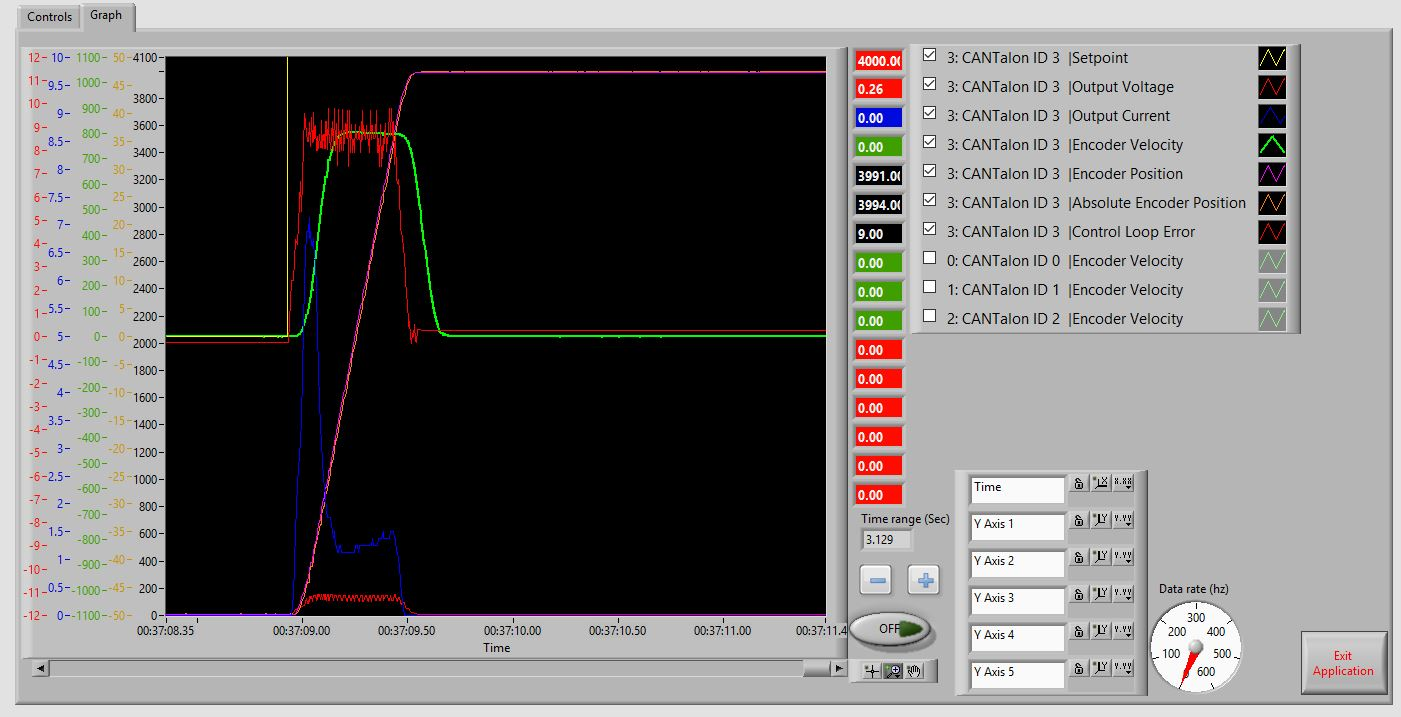
\includegraphics[scale=0.2]{assets/grapher}
\end{figure}

\begin{figure}[H]
	\centering
	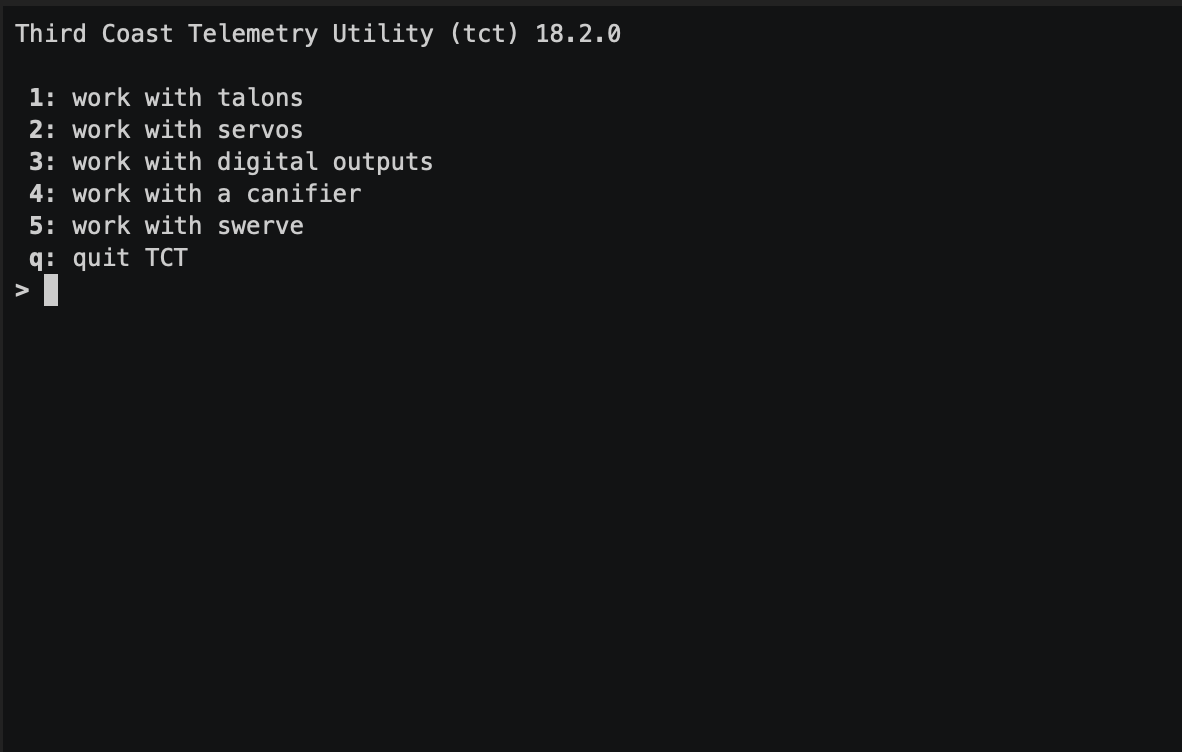
\includegraphics[scale=0.35]{assets/tct}
\end{figure}

Similar to the Grapher, \textbf{Keeper} logs data recorded from the robot during the execution of a command. The data is then made available through a Dash app using PostgreSQL and Plotly.

Stryke Force programmers are using a \textbf{Jupyter Notebook server} this year to test CV applications and algorithms, coordinate transformation math, and any other ideas that come to mind. All of our programmers have enjoyed the ease of logging in and being able to quickly test any idea anywhere.

\begin{figure}[H]
	\centering
	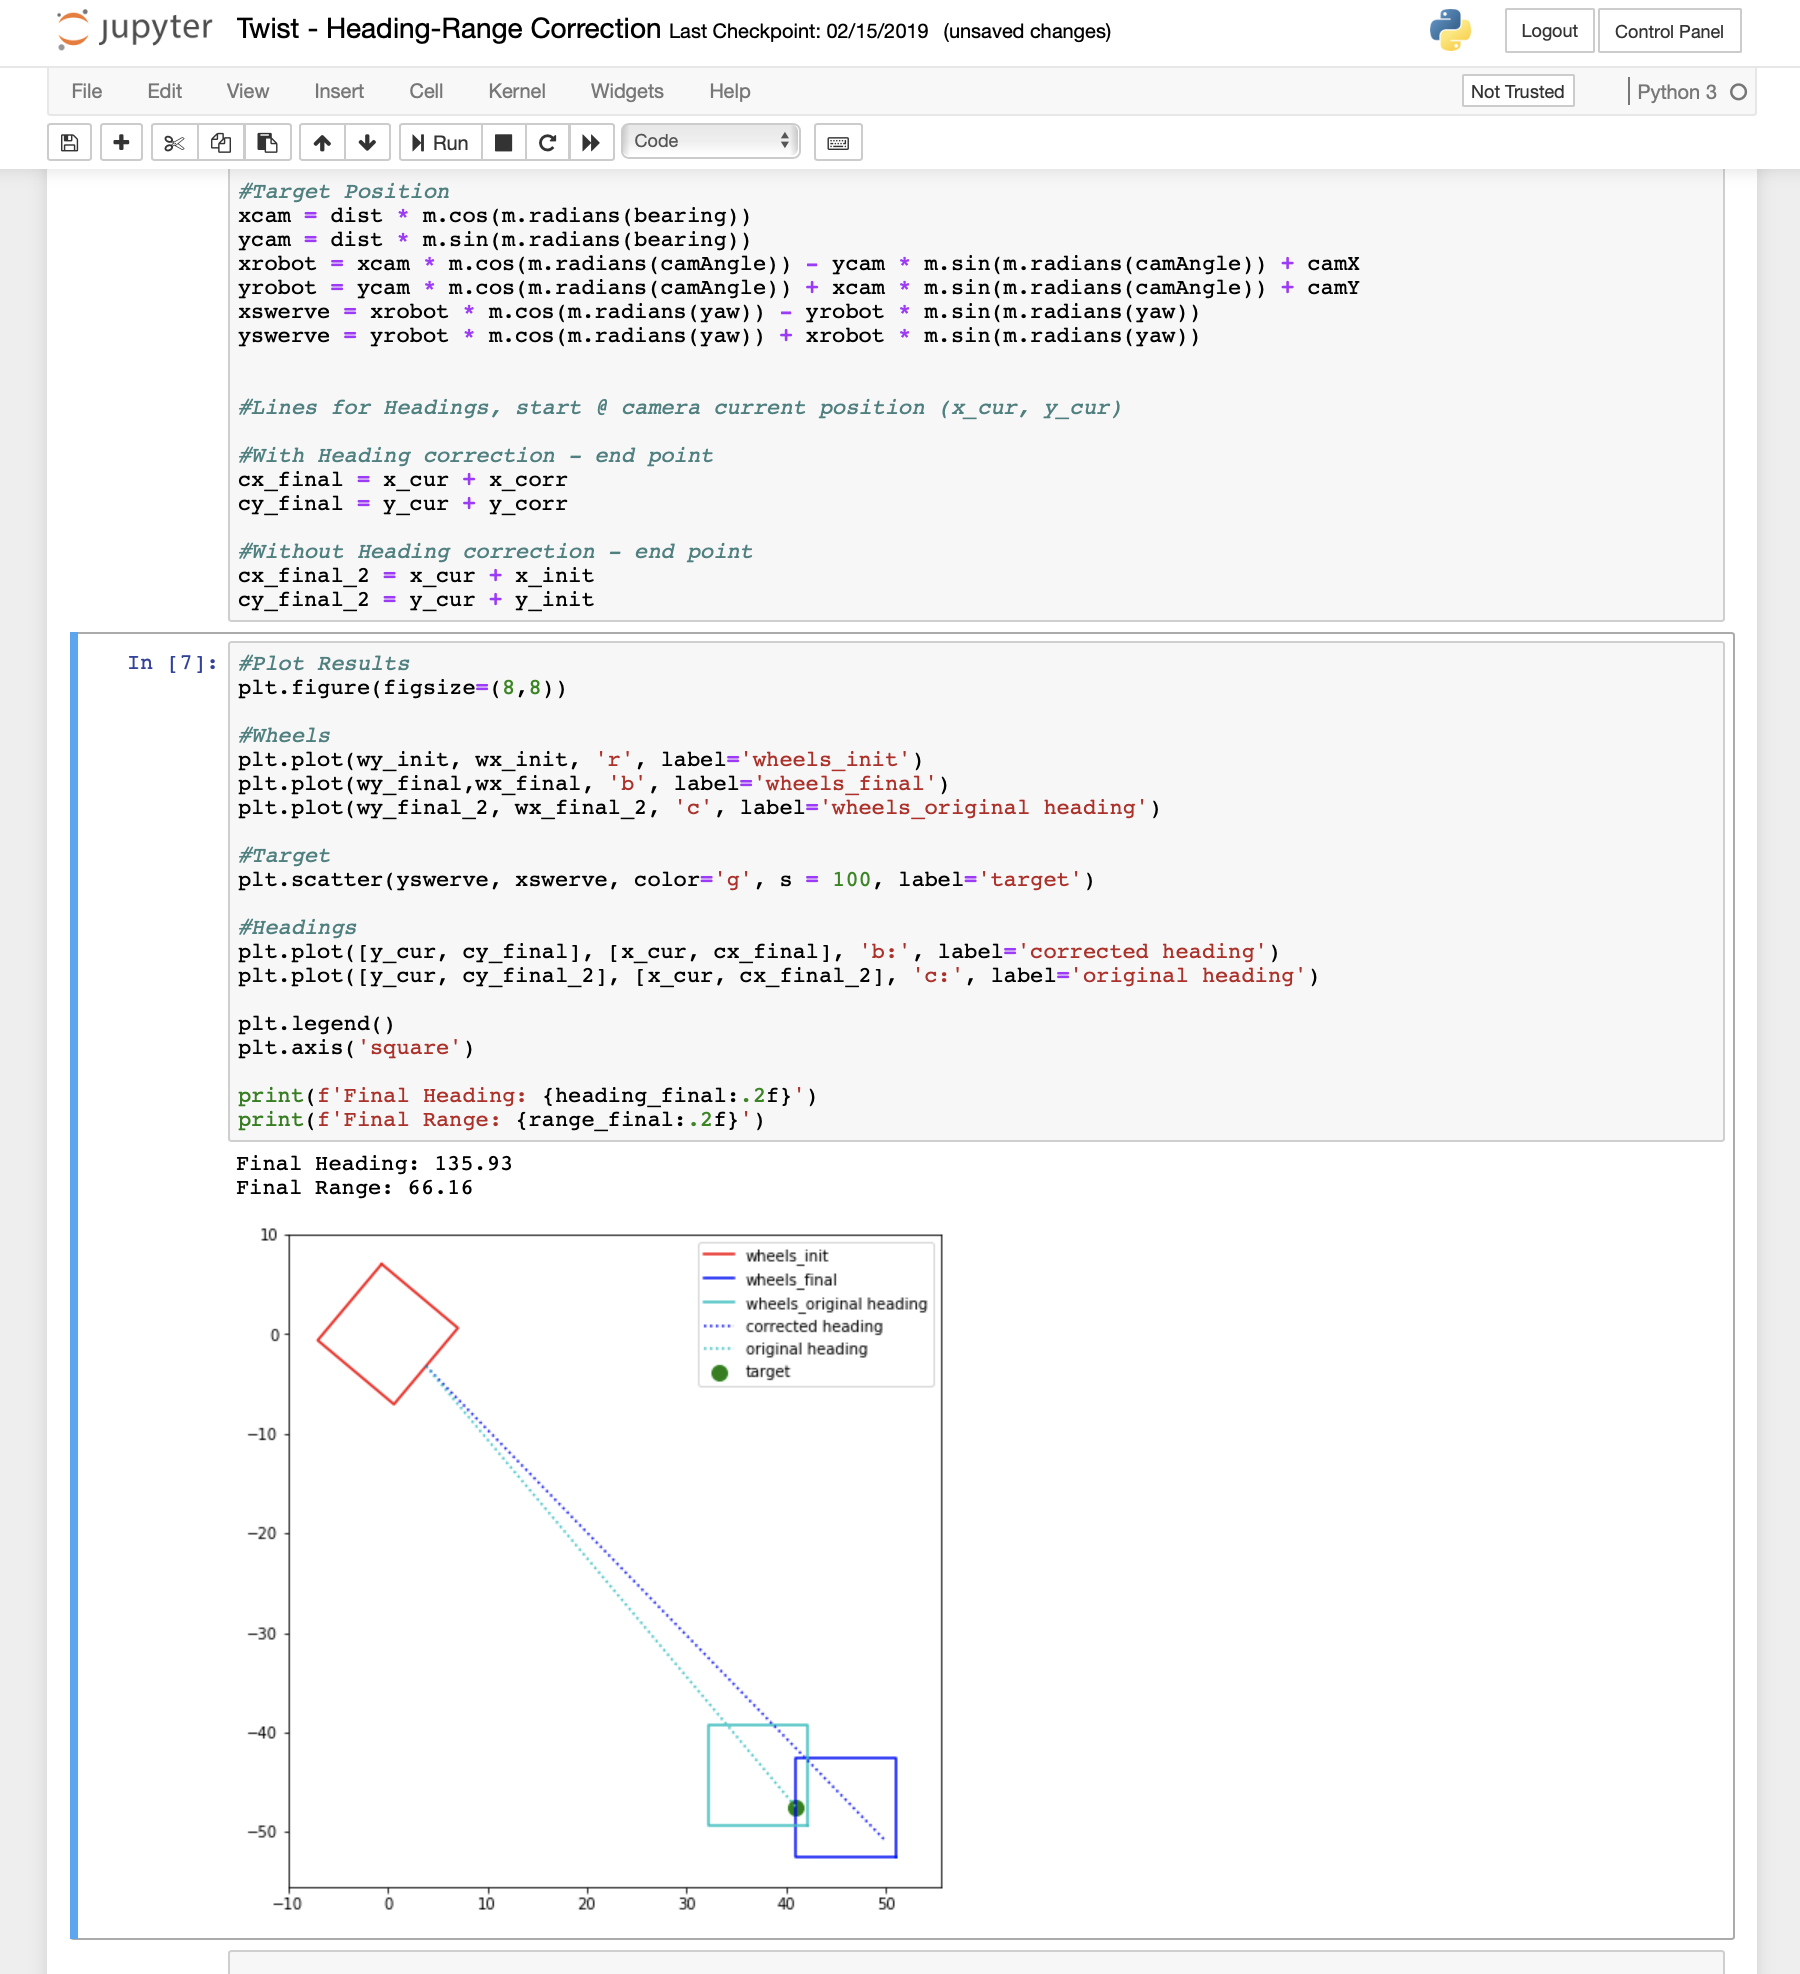
\includegraphics[scale=0.25]{assets/jupyter}
\end{figure}

\begin{figure}[H]
 \centering
% 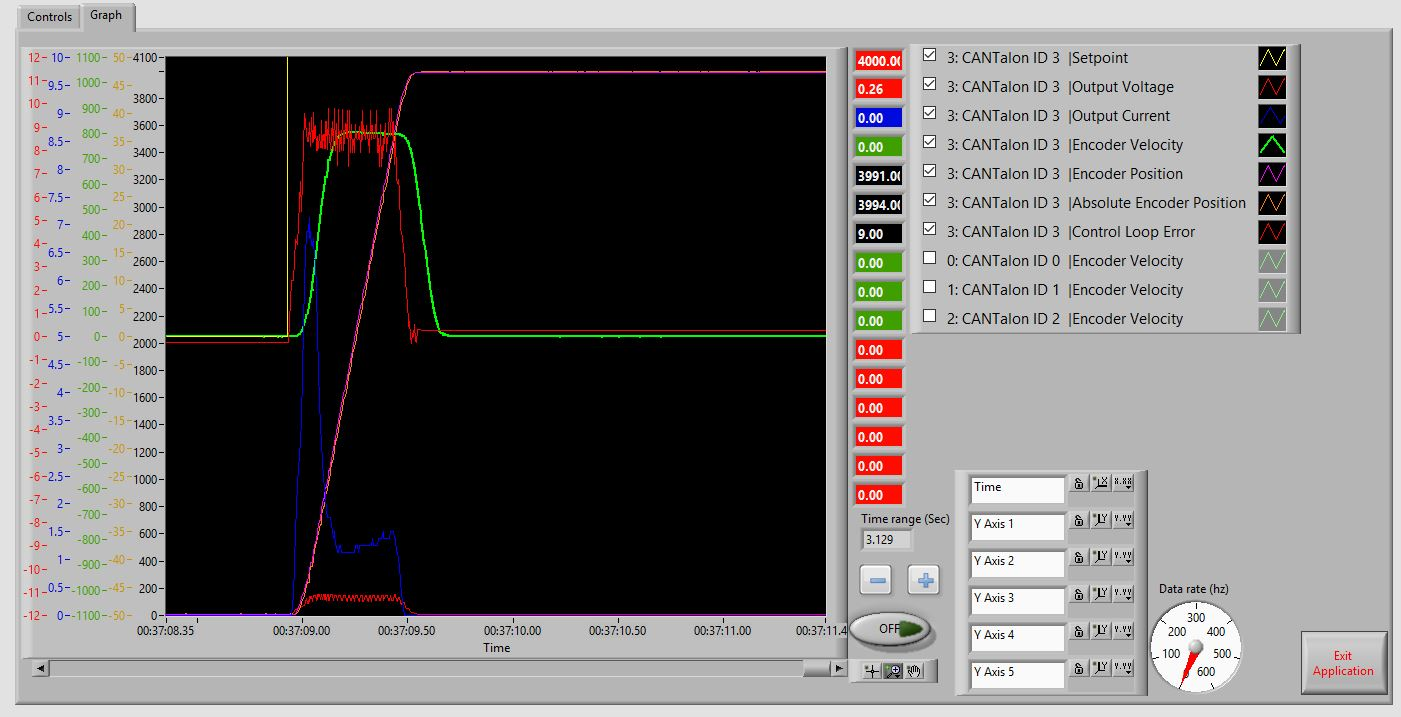
\includegraphics[scale=0.2]{assets/grapher}
\end{figure}

We are pleased to make TCT and the Grapher available as open source at https://github.com/strykeforce. More resources are available at https://www.strykeforce.org/resources.

\section{Software Engineering}

As members of Stryke Force, we learn how to work together using real-world tools and processes that will benefit us during college and our future careers.

This year’s \textit{FIRST}\textregistered DESTINATION: DEEP SPACE code is written in Java, an \textbf{object-oriented programming} language and leverages WPILib command-based programming. Our use of \textbf{system sequence diagrams} speeds up development and testing since all events are carefully planned in advance.

\begin{figure}[H]
	\centering
	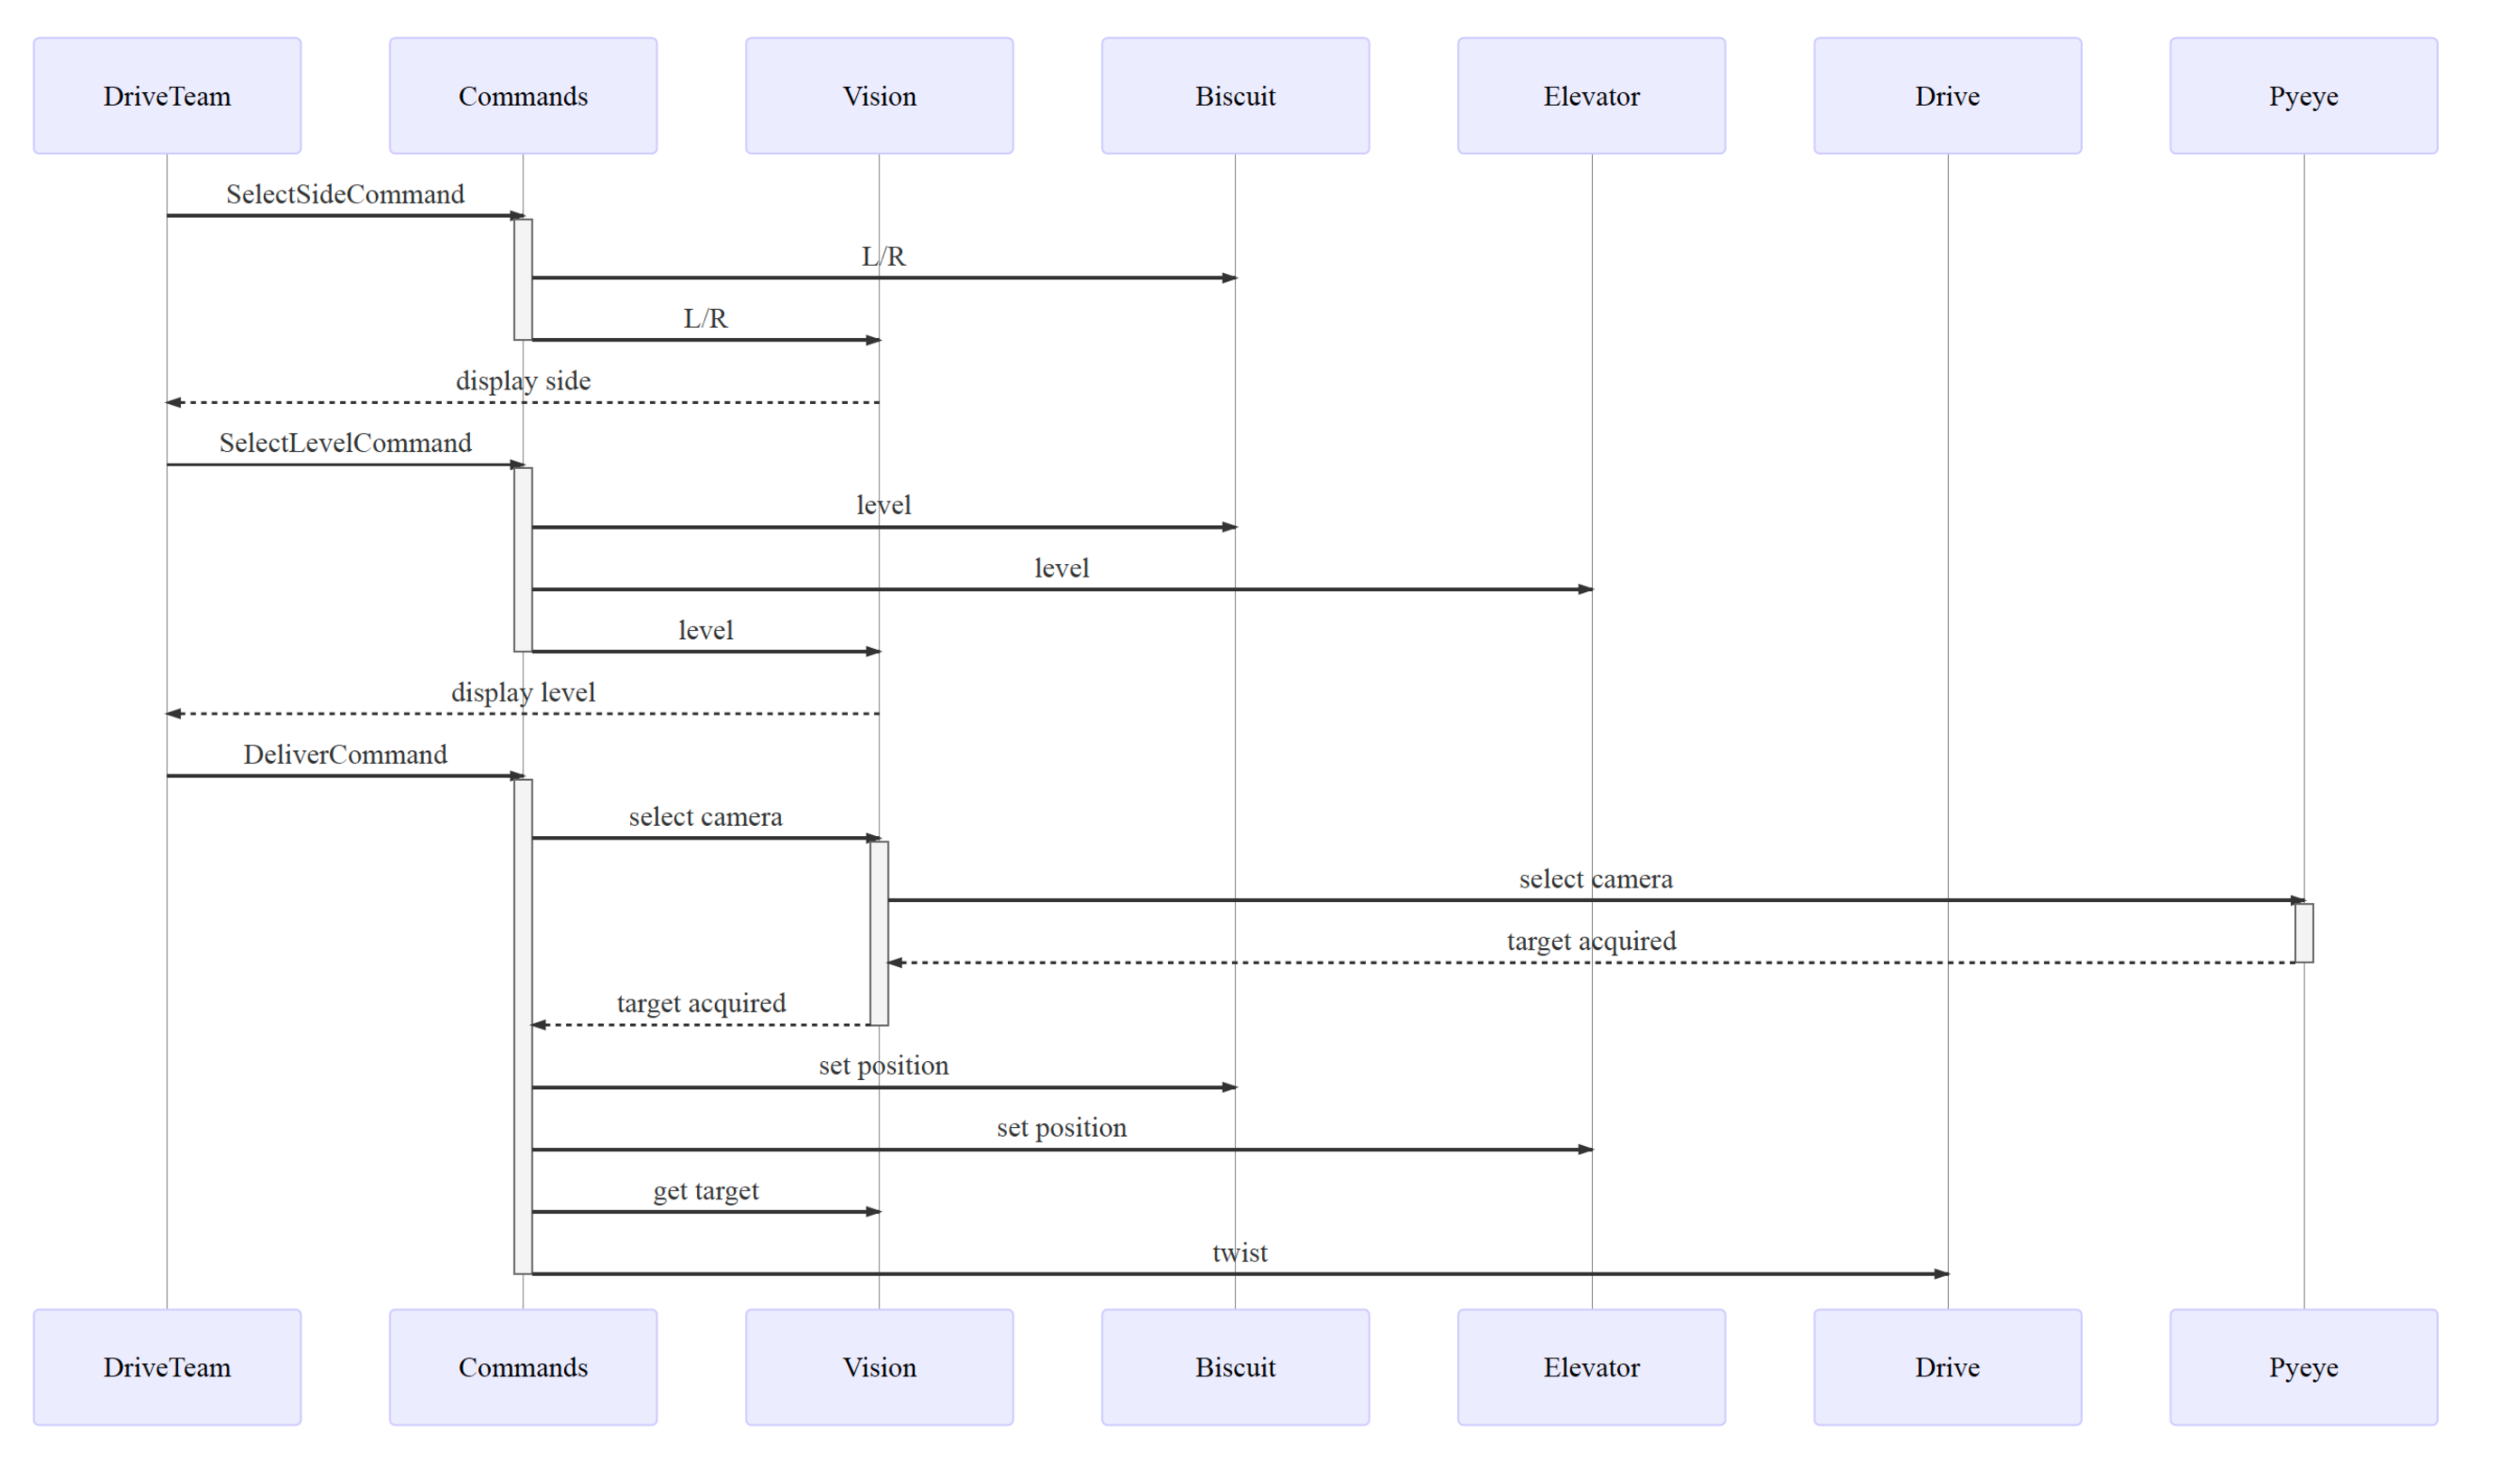
\includegraphics[scale=0.18]{assets/mermaid}
\end{figure}

The \textit{FIRST}\textregistered DESTINATION: DEEP SPACE and Pyeye projects use GradleRIO, the open-source build automation software. Stryke Force programmers use Gradle to build projects, deploy code to the RoboRIO, and manage dependencies.

Stryke Force uses GitHub and Git for version control. The programming team adopted the \textbf{OneFlow Git Branching Model and Workflow}.  The programmers maintain one master branch and create pull requests from feature branches.  For example, when working on autonomous paths, a programmer would create a new branch in which they would add and modify the autonomous code.  The programmer would then submit a pull request to the master branch in the Stryke Force repository. Pull requests undergo careful peer and mentor review before being merged into the master branch.

\end{document}